\documentclass[11pt,a4paper,faculty=we,language=en,doctype=report]{cls/ugent-doc}

% Optional: margins and spacing
%-------------------------------
% Uncomment and adjust to change the default values set by the template
% Note: the defaults are suggested values by Ghent University
%\geometry{bottom=2.5cm,top=2.5cm,left=3cm,right=2cm} 
%\renewcommand{\baselinestretch}{1.15} % line spacing
\setlength{\headheight}{13.59999pt}

% Font
%------
%\usepackage[T1]{fontenc}
\usepackage[utf8]{inputenc} % allows non-ascii input characters
\usepackage{tikz-feynman}
% Comment or remove the two lines below to use the default Computer Modern font
%\usepackage{libertine}
%\usepackage{libertinust1math}

\usepackage[sc]{mathpazo} %font or smth
\linespread{1.05}
\usepackage{microtype}

\usepackage{fancyhdr} % Headers and footers
\pagestyle{fancy} % All pages have headers and footers e.g contents above contents (except new ones)
\usepackage[Rejne]{fncychap} %fancy chapters
%options for chapters: Sonny, Lenny, Glenn, Conny, Rejne, Bjarne, Bjornstrup

% NOTE: because the UGent font Panno is proprietary, it is not possible to use it
% in Overleaf. But UGent does not suggest to use Panno for documents (or maybe only for
% the titlepage). For the body, the UGent suggestion is to use a good serif font (for
% LaTeX this could be libertine or Computer Modern).
\usepackage{slashed}

% Proper word splitting
%-----------------------
\usepackage[english]{babel} 

% Mathematics
%-------------
\usepackage{amsmath}
\usepackage{amsfonts}
\usepackage{mathrsfs}
% Figures
%---------
%\usepackage{graphicx} % optional: the package is already loaded by the template
\graphicspath{{./figures/}}
\usepackage{copyrightbox}
% Bibliography settings
%-----------------------
\usepackage{cite}

% Hyperreferences
%-----------------
\usepackage[colorlinks=true, allcolors=ugentblue]{hyperref}

% Whitespace between paragraphs and no indentation
%--------------------------------------------------
\usepackage[parfill]{parskip} 

% Input for title page
%----------------------

% The title
\thetitle{Radio detection of high energy neutrinos in the Greenland icecap}
\thesubtitle{Arthur Adriaens}

%% Note: a stricter UGent style could be achieved with, e.g.:
\usepackage{ulem} % for colored underline
\renewcommand{\ULthickness}{2pt} % adjust thickness of underline
\thetitle{\uline{\color{ugentblue}Radio detection of high energy neutrinos in the Greenland icecap}}
% Note: do not forget to reset the \ULthickness to 1pt after invoking \maketitle
% (otherwise all underlines in the rest of your document will be too thick):
%\renewcommand{\ULthickness}{1pt}

% The first (top) infobox at bottom of titlepage
\infoboxa{\bfseries\large Department of Physics and Astronomy}

% The second infobox at bottom of titlepage
\infoboxb{Promotor: 
\begin{tabular}[t]{ll}
    Prof. dr. Dirk Ryckbosch & Dirk.Ryckbosch@ugent.be\\ % note syntax 'short space'
\end{tabular}
}

% The third infobox at bottom of titlepage
\infoboxc{Accompanist: 
\begin{tabular}[t]{ll}
    Bob Oeyen &  Bob.Oeyen@ugent.be\\
\end{tabular}
}

% The last (bottom) infobox at bottom of titlepage
\infoboxd{Academic year: 2022--2023} % note dash, not hyphen
\infoboxd{Master’s dissertation submitted in partial fulfilment of the requirements for the degree of master in Physics and Astronomy}

\begin{document}

% =====================================================================
% Cover
% =====================================================================

% ------------ TITLE PAGE ---------
\maketitle
\renewcommand{\ULthickness}{1pt}

% =====================================================================
% Front matter
% =====================================================================

% ------------ TABLE OF CONTENTS ---------
{\hypersetup{hidelinks}\tableofcontents} % hide link color in toc
\newpage


% =====================================================================
% Main matter
% =====================================================================
\chapter{Foreword}
\section{Abstract: English}
The Radio Neutrino Observatory - RNO-G - is under construction at Summit Station in Greenland to search for neutrinos of several PeV energy up to the Eev range. It's a mid-scale, discovery phase, extremely high-energy neutrino telescope that will probe the astrophysical neutrino flux at energies beyond the reach of IceCube.
More particularly if will make it possible to reach the next major milestone in astroparticle physics: the discovery of cosmogenic neutrinos.
\vspace{0.5cm}
All simulations carried out within this work were made with the three programs 
\begin{itemize}
	\item NuRadioMC
	\item radiotools
	\item RadioPropa
\end{itemize}
whom are free to download on \href{https://github.com/nu-radio}{github}
\section{Abstract: Nederlands}
% =====================================================================
\chapter{Background}
\section{Standard model}
\begin{align*}
  \mathcal{L}_{SM} &= -\frac{1}{4}F^a_{\mu\nu}F^{\mu\nu a} - \frac{1}{4}G^a_ {\mu\nu}G^{\mu\nu a} - \frac{1}{4}B^a_ {\mu\nu}B^{\mu\nu a}\\
                   & + \sum_q \bar{\psi}_{q,L}(i\slashed{\mathcal{D}})\psi_{q,L} + \sum_l \bar{\psi}_{l,L}(i\slashed{\mathcal{D}})\psi_{l,L} + \sum_l \bar{\psi}_{q,R}(i\slashed{\mathcal{D}})\psi_{q,R} + \sum_l \bar{\psi}_{l,R}(i\slashed{\mathcal{D}})\psi_{l,R} \\
                   &+ \mathcal{D}_\mu \phi(\mathcal{D}^\mu \phi)^\dagger - u^2\phi\phi^\dagger - \lambda (\phi \phi^\dagger)^2\\
                   &+ g_Y^{(e)} \bar{\psi}_{e,L}\phi e_R + g_Y^{(u)}\bar{\psi}_{q,L}\tilde{\phi}u_R + g_Y^{(d)}\bar{\psi}_{q,L}\phi d_R+ h.c
\end{align*}
\subsection{V-A theory}
Fermi realised a quantitatively good local field theory for the $\beta$-decay in 1934 based on the idea of the following
interaction:
\begin{equation}
  n \rightarrow p + e^- + \bar{\nu}
\end{equation}
i.e
\begin{figure}
  \centering
  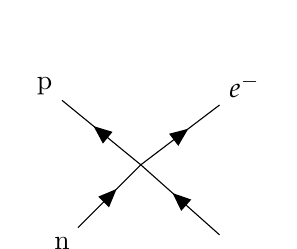
\begin{tikzpicture}
  \begin{feynman}
  \vertex (a0) {n};
  \vertex[right=1cm of a0] (ai);
  \vertex[right=1cm of ai] (a1) {\nu};
  \vertex[above=1cm of ai] (ii);
  \vertex[above=1cm of ii] (bi);
  \vertex[left=1cm of bi] (b0) {p};
  \vertex[right=1cm of bi] (b1) {$e^-$};
  \diagram* {
    {[edges=fermion]
      (a0) -- (ii) -- (b1)
    },
    {[edges=fermion]
      (a1) -- (ii) -- (b0)
    },
  };
  \end{feynman}
  \end{tikzpicture}
\end{figure}

\section{Discovery}
\subsection{See-saw mechanism}
Given a spinor $\psi$ with the following Lagrange density:
\begin{equation}
	\mathcal{L} = i\bar{\psi}\slashed{\partial}\psi - m\bar{\psi}\psi - \frac{M}{2} (\bar{\psi}_R\psi_{Rc} + \bar{\psi}_{Rc}\psi_R)
\end{equation}
We can re-write this Lagrangian in terms of
\begin{align}
	\chi &:= \frac{1}{\sqrt{2}} (\psi_R + \psi_{Rc})\\
	\omega &:= \frac{1}{\sqrt{2}} (\psi_L + \psi_{Lc})
\end{align}
by first identifying that
\begin{equation}
	- \frac{M}{2} (\bar{\psi}_R\psi_{Rc} + \bar{\psi}_{Rc}\psi_R)
\end{equation}
is equal to
\begin{equation}
	-M\bar{\chi} \chi = -\frac{M}{2} (\bar{\psi}_R + \bar{\psi}_{Rc}) (\psi_R + \psi_{Rc}) = -\frac{M}{2} (\bar{\psi}_R\psi_{Rc} + \bar{\psi}_{Rc}\psi_R)
\end{equation}
Where we've used
\begin{equation}
	\bar{\psi}_R\psi_{R} \equiv \psi_R^\dagger\gamma^0\psi_{R} \equiv P_R\psi^\dagger\gamma^0P_R\psi = P_RP_L\psi^\dagger\gamma^0\psi = 0
\end{equation}
And next that in
\begin{equation}
	i\bar{\psi}\slashed{\partial}\psi - m\bar{\psi}\psi = i\bar{\psi}_R\slashed{\partial}\psi_{R} + i\bar{\psi}_L\slashed{\partial}\psi_{L} - m\bar{\psi}_R\psi_{L} - m\bar{\psi}_L\psi_{R}
\end{equation}
We can identify that
\begin{align}
	\bar{\chi}\slashed{\partial}\chi &= \frac{1}{2}(\bar{\psi}_R\slashed{\partial}\psi_{R} + \bar{\psi}_{Rc}\slashed{\partial}\psi_{Rc}) = \bar{\psi}_R \slashed{\partial} \psi_{R}\\
	\bar{\omega}\slashed{\partial}\omega &= \bar{\psi}_L \slashed{\partial} \psi_{L}
\end{align}
Where we've done an integration by parts and used $\bar{\psi}_c\gamma_\mu\chi_c = -\bar{\chi}\gamma_\mu\psi$. We thus get:
\begin{equation}
	\mathcal{L} = i\bar{\chi}\slashed{\partial}\chi +i\bar{\omega}\slashed{\partial}\omega - m\bar{\psi}_R\psi_{L} - m\bar{\psi}_L\psi_{R} -M\bar{\chi} \chi 
\end{equation}
And finally we notice that
\begin{align}
	\bar{\chi}\omega &= \frac{1}{2} \left(\bar{\psi}_R\psi_L + \bar{\psi}_R\psi_{Lc} + \bar{\psi}_{Rc}\psi_{L} + \bar{\psi}_{Rc}\psi_{Lc}\right)\\
	&=  \frac{1}{2} \left(\bar{\psi}_R\psi_L + \bar{\psi}_R\psi_{Lc} + \bar{\psi}_{Rc}\psi_{L} + \bar{\psi}_{L}\psi_{R}\right)\\
	\bar{\omega}\chi &= \frac{1}{2} \left(\bar{\psi}_L \psi_{R} + \bar{\psi}_{Lc}\psi_{R} + \bar{\psi}_L\psi_{Rc} + \bar{\psi}_{Lc}\psi_{Rc}\right)\\
	&= \frac{1}{2} \left(\bar{\psi}_L \psi_{R} + \bar{\psi}_{Lc}\psi_{R} + \bar{\psi}_L\psi_{Rc} + \bar{\psi}_{R}\psi_{L}\right)
\end{align}
As $\bar{\psi}_c\chi_c = \bar{\chi}\psi$. Summing these, we get:
\begin{align}
	\bar{\chi}\omega + \bar{\omega}\chi &= \bar{\psi}_L \psi_R + \bar{\psi}_R \psi_{L}\\
	&\quad + \frac{1}{2}\left(\bar{\psi}_R\psi_{Lc} + \bar{\psi}_{Rc} \psi_{L} + \bar{\psi}_{Lc}\psi_R + \bar{\psi}_L\psi_{Rc}\right)\\
	&= \bar{\psi}_L \psi_R + \bar{\psi}_R \psi_{L}
\end{align}
Where we've used the handedness flips a charge conjugation entails, at last we now have:
\begin{equation}
	\mathcal{L} = i\bar{\chi}\slashed{\partial}\chi +i\bar{\omega}\slashed{\partial}\omega - m(\bar{\chi}\omega + \bar{\omega}\chi) -M\bar{\chi} \chi 
\end{equation}
Now to determine the mass eigenstates we'll re-write this equation into the form
\begin{equation}
	\mathcal{L} = i\bar{\chi}\slashed{\partial}\chi +i\bar{\omega}\slashed{\partial}\omega 
	-\left(\begin{array}{cc}
		\bar{\chi} &\bar{\omega}
	\end{array}\right)\cdot
	\left(\begin{array}{cc}
		M & m \\
		m & 0
	\end{array}\right) \cdot \left(\begin{array}{c}
	\chi \\ \omega
\end{array}\right)
\end{equation}
lets now find the eigenvalues:
\begin{equation}
	\left| \begin{array}{cc}
		M-\lambda & m \\
		m & -\lambda
	\end{array} \right| = (\lambda-M)\lambda - m^2 = 0 \implies \lambda_\pm  = \frac{M\pm \sqrt{M^2 + 4m^2}}{2} \label{eigenvalues}
\end{equation}
i.e
\begin{equation}
	\lambda_\pm = \frac{M}{2}\left( 1 \pm \sqrt{1 + 4m^2/M^2}\right)
\end{equation}
Now we'll determine the eigenvectors:
\begin{equation}
\left[\begin{array}{cc}
	M-\lambda_\pm & m \\
	m & -\lambda_\pm
\end{array}\right] \left(\begin{array}{c}
x_\pm \\
y_\pm
\end{array}\right) = \vec{0}
\end{equation}
this gives
\begin{align}
	Mx_\pm - \lambda_\pm x_\pm + my_\pm &= 0\\
	m x_\pm - \lambda_\pm y_\pm &= 0 \implies \frac{m x_\pm}{\lambda_\pm} = y_\pm
\end{align}
inserting the second equation in the first we get:
\begin{align}
	Mx_\pm - \lambda_\pm x_\pm + m \frac{m x_\pm}{\lambda_\pm} = 0 &= M\lambda_\pm x_\pm - \lambda_\pm^2 x_\pm + m^2 x_\pm\\
	&= x_\pm(\lambda_\pm^2 -M\lambda_\pm + m^2)
\end{align}
which is true for every $x_\pm$ (see equation \ref{eigenvalues}) i.e we can freely choose $x_\pm$ so let's opt for $x_\pm^2 + y_\pm^2 = 1$:
\begin{align}
	x_\pm^2(1+\frac{m^2}{\lambda_\pm^2}) = 1 \implies x^2_\pm = \frac{1}{1+\frac{m^2}{\lambda_\pm^2}} \implies x_\pm &= \frac{\lambda_\pm}{\sqrt{\lambda_\pm^2 + m^2}}\\
	\& \quad y_\pm &= \frac{m}{\sqrt{\lambda_\pm^2 + m^2}}
\end{align}
And thus, summing up, we get the eigenvectors $\phi_\pm$ with eigenvalues $m_\pm$:
\begin{equation}
	\phi_\pm := \left(\begin{array}{c}
		x_\pm\\
		y_\pm
	\end{array}\right) = \left(\begin{array}{c}
		\frac{\lambda_\pm}{\sqrt{\lambda_\pm^2 + m^2}}\\
		\frac{m}{\sqrt{\lambda_\pm^2 + m^2}}
	\end{array}\right) \quad \text{ and }\quad m_\pm := \lambda_\pm =  \frac{M}{2}\left( 1 \pm \sqrt{1 + 4m^2/M^2}\right)
\end{equation}
Now we'll consider the limit $M \gg m$:
\begin{equation}
	m_\pm =  \frac{M}{2}\left( 1 \pm \sqrt{1 + 4m^2/M^2}\right) \approx \frac{M}{2}\left(1\pm1\pm\frac{2m^2}{M^2}\right)
\end{equation}
Which gives:
\begin{align}
	m_+ &\approx M\\
	m_- &\approx -\frac{m^2}{M}
\end{align}
and:
\begin{align}
	\phi_+&\approx \left(\begin{array}{c}
		\frac{M}{M}\\
		\frac{m}{M}
	\end{array}\right) = \left(\begin{array}{c}
	1\\
	m/M
	\end{array}\right)\\
	\phi_-&\approx \left(\begin{array}{c}
		-\frac{m}{M}\\
		\frac{m}{m}
	\end{array}\right) = \left(\begin{array}{c}
		-m/M\\
		1
	\end{array}\right)
\end{align}
i.e, in the $\chi,\omega$ basis:
\begin{align}
	m_+\approx M \quad &\text{with eigenstate} \quad \chi + \frac{m}{M}\omega\\
	m_-\approx -\frac{m^2}{M} \quad &\text{with eigenstate} \quad  \omega - \frac{m}{M}\chi\\
\end{align}
Here we can clearly see the See-Saw mechanism at work, for a certain $m$ if we choose a big $M$ we'll get a big $m_+$ and small $m_-$ (and vice versa). We also see that there's only a very small mixing of states, i.e the $m_-$ mass state is almost purely $\omega$ (and $m_+$ almost purely $\chi$). The parameter $m$ in the original matrix is forbidden by electroweak gauge symmetry, and can only appear after the symmetry has been spontaneous broken by a Higgs mechanism; for this reason a good estimate of the order of $m$ is the vaccuum expectation energy: $m\approx v = 246 \approx 10^2$GeV. In grand unified theories it's theorised that $M\approx 10^{15}$GeV after symmetry breaking, using these values we get
\begin{align}
	m_- \approx 10^{-11}\text{GeV} \approx 10^{-2} \text{eV}
\end{align}
which is an appropriate mass size for the observed neutrinos
\section{Why?}
Neutrinos are ideal messengers to identify the UHE (Ultra High Energy) sources
in the universe. Unlike cosmic rays, which are deflected by magnetic fields and
interact with matter and radiation on their way to us, neutrinos point back to
sources and can reach Earth unperturbed from the most distant corners of the
universe.  Neutrinos can be generated in 2 ways: either they're generated in
interactions at the sources, termed \textit{astrophysical neutrinos}. Or
they're created through the interaction of ultra-high energy cosmic rays during
propagation with the cosmic microwave or other photon backgrounds termed
\textit{cosmogenic neutrinos}. 
Supernovae are a source for \textit{astrophysical neutrinos}:
\subsection{Supernovae}
A star starts its life as a ball of pure hydrogen, at the core due to the
gravitational pressure of the outside plasma fusion of hydrogen into deuterium
and helium happens, converting mass into energy. The pressure of this energy
counteracts the pressure of gravity and the star is stable.

When the hydrogen at the core runs out no more hydrogen can be fused and the
fusion of heavier elements starts, this can't keep going on however as at some
point the star starts to form the most stable element: iron.  It costs energy
to both make lighter elements than iron and heavier ones.  As the iron core
builds up the outside pressure from the core starts to decrease as no new
energy is released. This goes on until the inwards pressure becomes too large
and the electrons surrounding the iron core fuse with the protons, 
creating neutrons and neutrino's.

This last part happens in a split second, creating a very dense neutron star
and up to $10^{52}$ ultra-relativistic neutrinos. As the density has suddenly
increased so much there's a huge distance of pure vaccuum between the plasma
outer layer and the (now) neutron star, this plasma starts falling in as these
neutrinos carrying tremendous amounts of energy start going outwards the neutron
stars core.

These then collide resulting in what we observe as a "supernova", wrongly
thought of by Kepler as being a "new (nova) star" rather being a violent death
of an old star.

Not all the neutrinos collide with matter of course as neutrinos rarely
interact, it's only as the incoming plasma is so dense and due to the
tremendous amount of neutrinos that collissions happen at all. The ones that
escape, however, will be visible on earth in our neutrino detectors, far before
the light escapes the exploding star.

Neutrino observatories are thus useful to know where to point our various
telescopes before the supernova is actually visible in the night sky.
\subsection{Oscillations}
\subsection{Majorana}
\section{Outside sources}
The radio detection of neutrinos targets the energy range 10PeV to 100EeV\cite{Aguilar_2021}, here we'll see diffuse neutrino fluxes both directly from sources (\textit{astrophysical neutrinos}) i.e created directly in (or very close to) the sources of ultra-high energy cosmic rays (UHECRs), as well as from the interaction of UHECRs with photon backgrounds (e.g the CMB) (\textit{cosmogenic neutrinos}).
\subsection{primordial neutrinos}
To estimate the temperature of the neutrinos who decoupled at the start of the universe, we can take a look at conservation of entropy \cite{Dodelson}
(...)
The entropy before and after decoupling are:
\begin{align}
	s(a_1) &= \frac{2\pi^2}{45}(2 + \frac{7}{8}(2+2+3+3))T_1^3\\
	&= \frac{2\pi^2}{45}\frac{86}{8}T_1^3\\
	s(a_2) &= \frac{2\pi^2}{45}(2T_\gamma^3 + \frac{7}{8}(6)T_\nu^3)\\
\end{align}
Conservation of entropy:
\begin{align}
	s(a_1)a_1^3 &= s(a_2)a_2^3\\
	\frac{86}{8}(T_1 a_1)^3 &= \left(2\left(\frac{T_\gamma}{T_\nu}\right)^3 + \frac{42}{8}\right)(T_\nu a_2)^3\\
	\frac{86}{8} &= 2\left(\frac{T_\gamma}{T_\nu}\right)^3 + \frac{42}{8}\\
	\frac{44}{16} &= \left(\frac{T_\gamma}{T_\nu}\right)^3\\
	\left(\frac{T_\gamma}{T_\nu}\right) &= \left(\frac{11}{4}\right)^{1/3}
\end{align}
i.e
\begin{equation}
	T_\nu = \left(\frac{4}{11}\right)^{1/3}T_\gamma
\end{equation}
\section{Why look for them?}
The origin of the most energetic cosmic rays is still not conclusively identified. One approach to solving this problem is \textit{multi-messenger astrophysics}, where several types of cosmic particles are used to identify the sources of these ultra-high energy cosmic rays (UHECRs). E.g we simultaneously measure gravitational waves (gravitons?) with the Einstein telescope, neutrino's with IceCube (or eventually RNO-G) and muons with a muon detector.
\newpage
\chapter{Radio detection}
For a particle shower to emit strong radio signals, two conditions have to be met:
\begin{itemize}
	\item There needs to be a speration of positive and negative charges in the shower front 
	\item The signals produced over the length of the shower profile need to overlap coherently.
\end{itemize}
The first item, seperation of positive and negative charges, can be caused by 2 mechanisms: The \textit{Askaryan} effect\cite{Askaryan}, also known as Askaryan radiation. This is the phenomenon whereby a particle traveling faster than the phase velocity of light in a dense dielectric (such as ice) produces a shower of secondary charged particles which contains a charge anisotropy (net negative charge), this charge imbalance is a result of medium electrons either Compton scattering into the advancing shower or annihilating with shower positrons. You thus get moving charges which move faster than the light speed in the medium, creating Cherenkov radiation.
The other effect, called \textit{geomagnetic emission} is the seperation of charges by the Lorentz force from the geomagnetic field, however, because of its relatively high density, in ice the Askaryan effect is dominant.
It's possible to distinguish between the two with polarization as with Askaryan emission, the light is polarized in the radial direction towards the shower axis contrary to geomagnetic emission where it's polarized in the Lorentz force direction.

In the following two sections I'll quickly give a short overview of the equations of Cherenkov radiation to determine the viewing angle of an incoming neutrino particle, this is relevant to the second condition which I'll explain afterwards. The reader who wants a thorough explanation and derivation is advised to check out \textit{Chapter 14: Radiation by Moving Charges} from the book \textit{Classical Electrodynamics} by Jackson. 
\section{Spectral distribution of radiation}
We wish to know the emitted energy per elementary unit solid angle over a certain frequency interval for a moving charge far away from the source. For this we have that the vectorpotential $\mathbf{A}$, defined as
\begin{equation}
	\mathbf{B} = \mathbf{\nabla}\times \mathbf{A}
\end{equation}
takes the form
\begin{equation}
	\mathbf{A}(\omega) = \frac{q}{4\pi \sqrt{2\pi}} \sqrt{\frac{\mu}{\epsilon}} \frac{e^{ikr}}{r} \boldsymbol{\alpha}
\end{equation}
with q the charge, r the distance from the charge to the observer and 
\begin{equation}
	\boldsymbol{\alpha} = \int_\infty^\infty \boldsymbol{\beta}(t) e^{i\omega(t-\boldsymbol{e}_r\cdot \boldsymbol{r}_0(t)/c')}\text{d}t
\end{equation}
With $\boldsymbol{\beta}:= \boldsymbol{u}/c'$ wherein $\boldsymbol{u}$ is the speed of the particle, $c'$ is the local speed of light and the integration is along the path of the moving charged particle. 
The energy emitted per unit solid angle is given by
\begin{equation}
	\frac{\text{d} \mathscr{P}}{\text{d} \Omega} = R'^2\mathbf{S}(t)\cdot\mathbf{n}'
\end{equation}
Defining $\mathscr{E}$ to be the time integral of this, we can reformulate this into (standard practice to integrate over the frequencies)
\begin{equation}
	\frac{\text{d} \mathscr{E}}{\text{d} \Omega} = r^2\int_\infty^\infty \text{d}\omega (\mathbf{E}(\omega)\times\mathbf{H}(-\omega))\cdot\mathbf{e}_r  = \int_0^\infty \frac{\text{d}^2 \mathscr{J}(\omega)}{\text{d} \omega \text{d} \Omega}
\end{equation}
i.e $\frac{\text{d}^2 \mathscr{J}}{\text{d}\omega \text{d}\Omega}$ is the energy radiated per elementary unit solid angle and per elementary unit frequency interval, re-writing gives
\begin{equation}
	\frac{\text{d}^2 \mathscr{J}(\omega)}{\text{d} \omega \text{d} \Omega} = 2r^2 \Re\{\mathbf{E}(\omega)\times\mathbf{H}^*(\omega)\}\cdot\mathbf{e}_r 
\end{equation}
up to $\mathcal{O}(r^{-2})$ we get
\begin{equation}
	\frac{\text{d}^2 \mathscr{J}(\omega)}{\text{d} \omega \text{d} \Omega} = \frac{q^2\omega^2}{16\pi^3}\sqrt{\frac{\mu}{\epsilon}}|\mathbf{e}_r\times(\mathbf{e}_r\times\boldsymbol{\alpha})|^2\label{equation: 4.123 in elektromagnetisme}
\end{equation}
\section{Cherenkov radiation}
Cherenkov radiation is like the elektromagnetic equivalent of a sonic boom, a sonic boom happens when something goes faster than the sounds speed in the medium; A particle emits Cherenkov radiation if it goes faster than the light speed in the medium. Choosing the particle trajectory to lie along the z axis we can approximate equation \ref{equation: 4.123 in elektromagnetisme} as
\begin{equation}
	\frac{\text{d}^2 \mathscr{J}(\omega)}{\text{d} \omega \text{d} \Omega} = \frac{q^2}{4\pi}\sqrt{\frac{\mu}{\epsilon}}\beta^2\omega^2\delta^2[\omega(1-\beta \mathbf{e}_r\cdot\mathbf{e}_z)]|\mathbf{e}_r\times\mathbf{e}_z|^2 \label{equation: 4.128 in elektromagnetisme}
\end{equation}
or, in spherical coordinates, $1-\beta \mathbf{e}_r\cdot\mathbf{e}_z = 1-\beta\cos(\theta_c)$ in the delta function. We thus only expect radiation if
\begin{equation}
\cos(\theta_c) = \frac{1}{\beta} = \frac{c'}{u} = \frac{c}{n}\cdot\frac{1}{u}
\end{equation}
I.e if $u>\frac{c}{n}$ with n the index of refraction, Cherenkov radiation will be emitted along a cone surface with half angle $\frac{\pi}{2}-\theta_c$ as illustrated in figure \ref{figure: Cherenkov illustratie}. Integrating equation \ref{equation: 4.128 in elektromagnetisme} over the solid angle and formally deviding by the time interval we get:
\begin{equation}
	\frac{\text{d}^2\mathscr{J}}{\text{d}\omega \text{d}t} = \frac{q^2}{4\pi}\sqrt{\frac{\mu}{\epsilon}}\beta\omega\left(1-\frac{1}{\beta^2}\right)	
\end{equation}
We see that the energy is proportional to $\omega$, so we expect that most radiation will be emitted "in blue", as seen in figure \ref{figure: Cherenkov reactor}.
For ice the index of refraction is roughly 1.75, so we expect an ultra-relativistic particle to produce the most radiation at around 55° opening as $\cos\left(\frac{1}{1.75}\right)\approx 55$° (generally we take 56°).
\begin{figure}
\centering
\begin{minipage}{0.45\textwidth}
	\centering
	\copyrightbox[r]{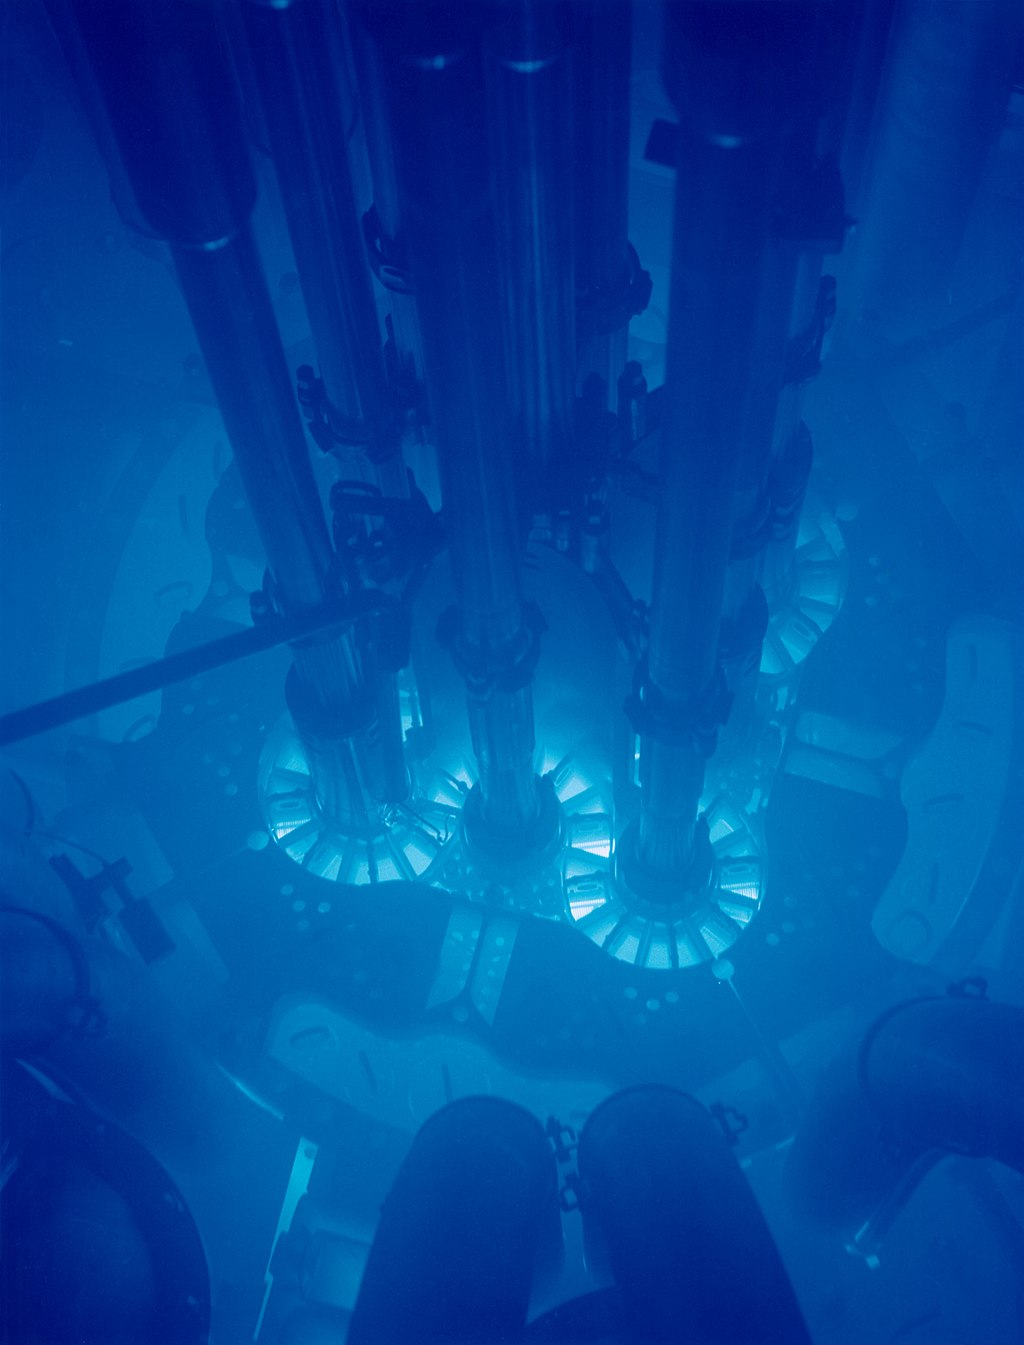
\includegraphics[height = 0.8\textwidth]{Cherenkov-reactor.jpg}}{\textcopyright Argonne National Laboratory\\Advanced Test Reactor core, Idaho National Laboratory}
	\caption{Cherenkov radiation in a nuclear reactor}
	\label{figure: Cherenkov reactor}
\end{minipage}
\hspace{0.05\textwidth}
\begin{minipage}{0.45\textwidth}
	\centering
	\copyrightbox[r]{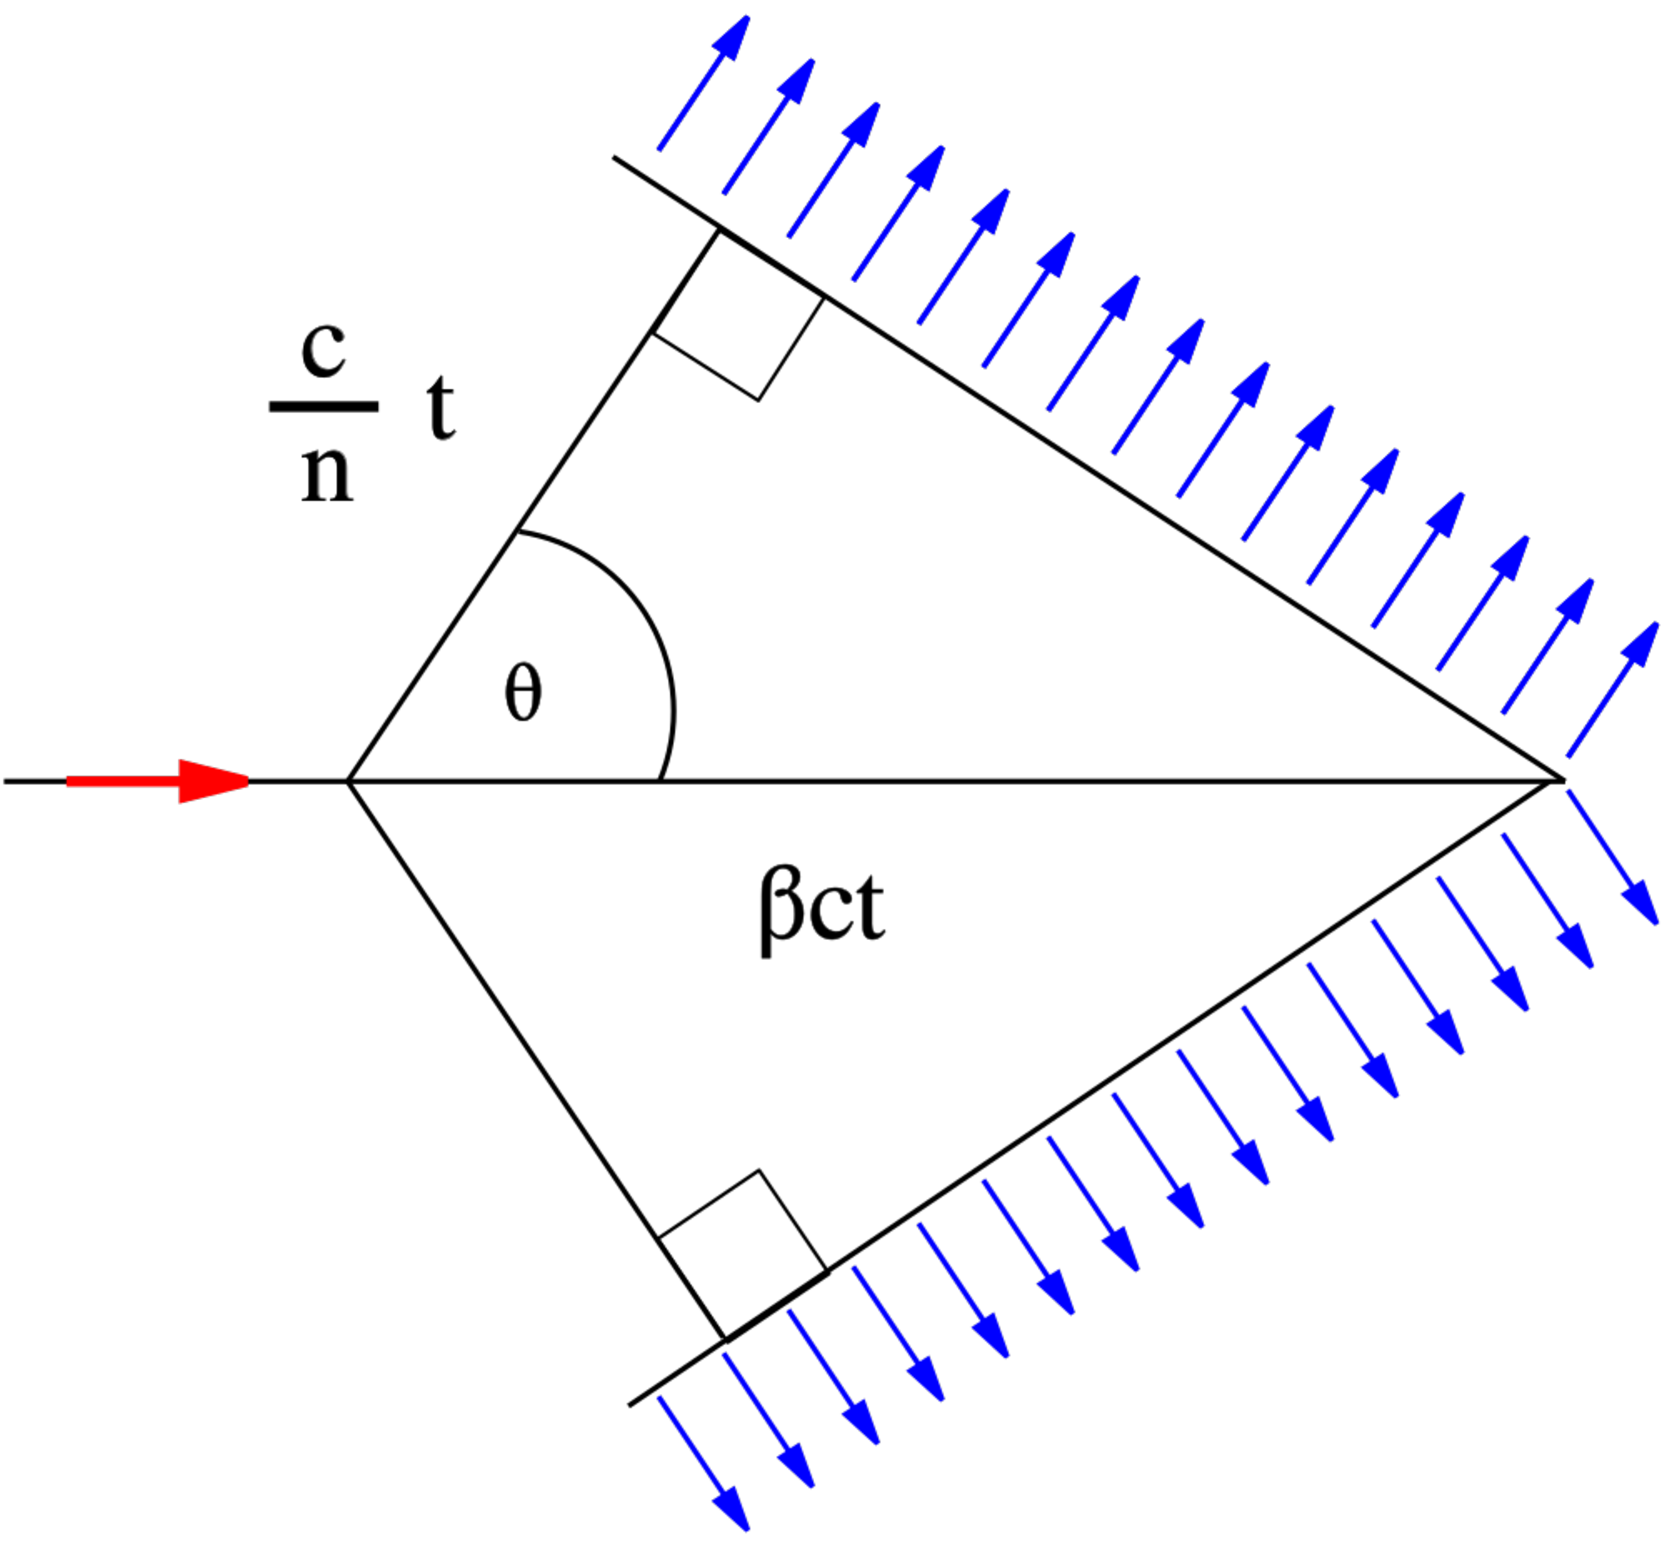
\includegraphics[height = 0.8\textwidth]{Cherenkov.pdf}}{\textcopyright Arpad Horvath}
	\caption{Diagrammatic representation of Cherenkov radiation}
	\label{figure: Cherenkov illustratie}
\end{minipage}
\end{figure}
Now if an observer is positioned at this Cherenkov angle all radio emission produced during the shower development reaches him/it at the same time, leading to constructive interference, hence the second condition is satisfied in ice for signals of $\approx 56°$
\section{Reconstruction}
It can pose a challenge to reconstruct the radio signals produced by the Cherenkov radiation as they are often obscured by background noise. A solution used in RadioReco is Information Field Theory (IFT) implemented in RadioReco by Welling et al.\cite{Welling_2021} which uses Bayesian inference to calculate the most likely radio signal, given recorded data.
\chapter{The Detector}
Both cosmic ray and neutrino detectors face the same main problem at the highest energies: the steeply falling flux requires large effective areas, wich leads to the construction of neutrino detectors with volumes on the cubic kilometer scale: IceCube. As we wish to detect neutrino's with even higher energies we turn to look at an array of detectors spanning multiple cubic kilometers: RNO-G.

One such detector is illustrated in figure \ref{fig:detector}.

The deep component of the detector can be split up in three parts: Two \textit{helper strings}, one \textit{power string} and the surface components. The helper strings are the 2 vertical cables shown on the right of the figure and each house 2 vertically polarized antennas (Vpols), one quadslot antenna for the horizontal polarization component (Hpol) and one radio pulser on each helper string which can be used to generate calibration signals.

The power string (the leftmost vertical cable) is more densely instrumented: At the bottom it houses a set of four Vpol and two Hpol antennas with a spacing of 1m and further up the string, with a spacing of 20m are three more Vpol antennas.

The signal from each of these antennae are fed into a low-noise amplifier directly above it, from there the signal is send to the data acquisition (DAQ) system at the surface via a Radio Frequency over Fiber (RFoF) cable. There it's again amplified, digitized and saved onto an SD card. This data is then transmitted via a Long Term Evolution (LTE) telecommunications network to a local server\footnote{There is additionally a Long Range Wide Area Network (LoRaWAN) antenna as backup in case of problems with the LTE network}, from where it is sent via a sattelite link.

There are solar panels as a power source who charge up battery banks, but as there is't enough light during the Greenland winters, there're plans to build wind turbines (with the problem being the possibly detectable RF noise the 'engine' produces)

\begin{figure}
	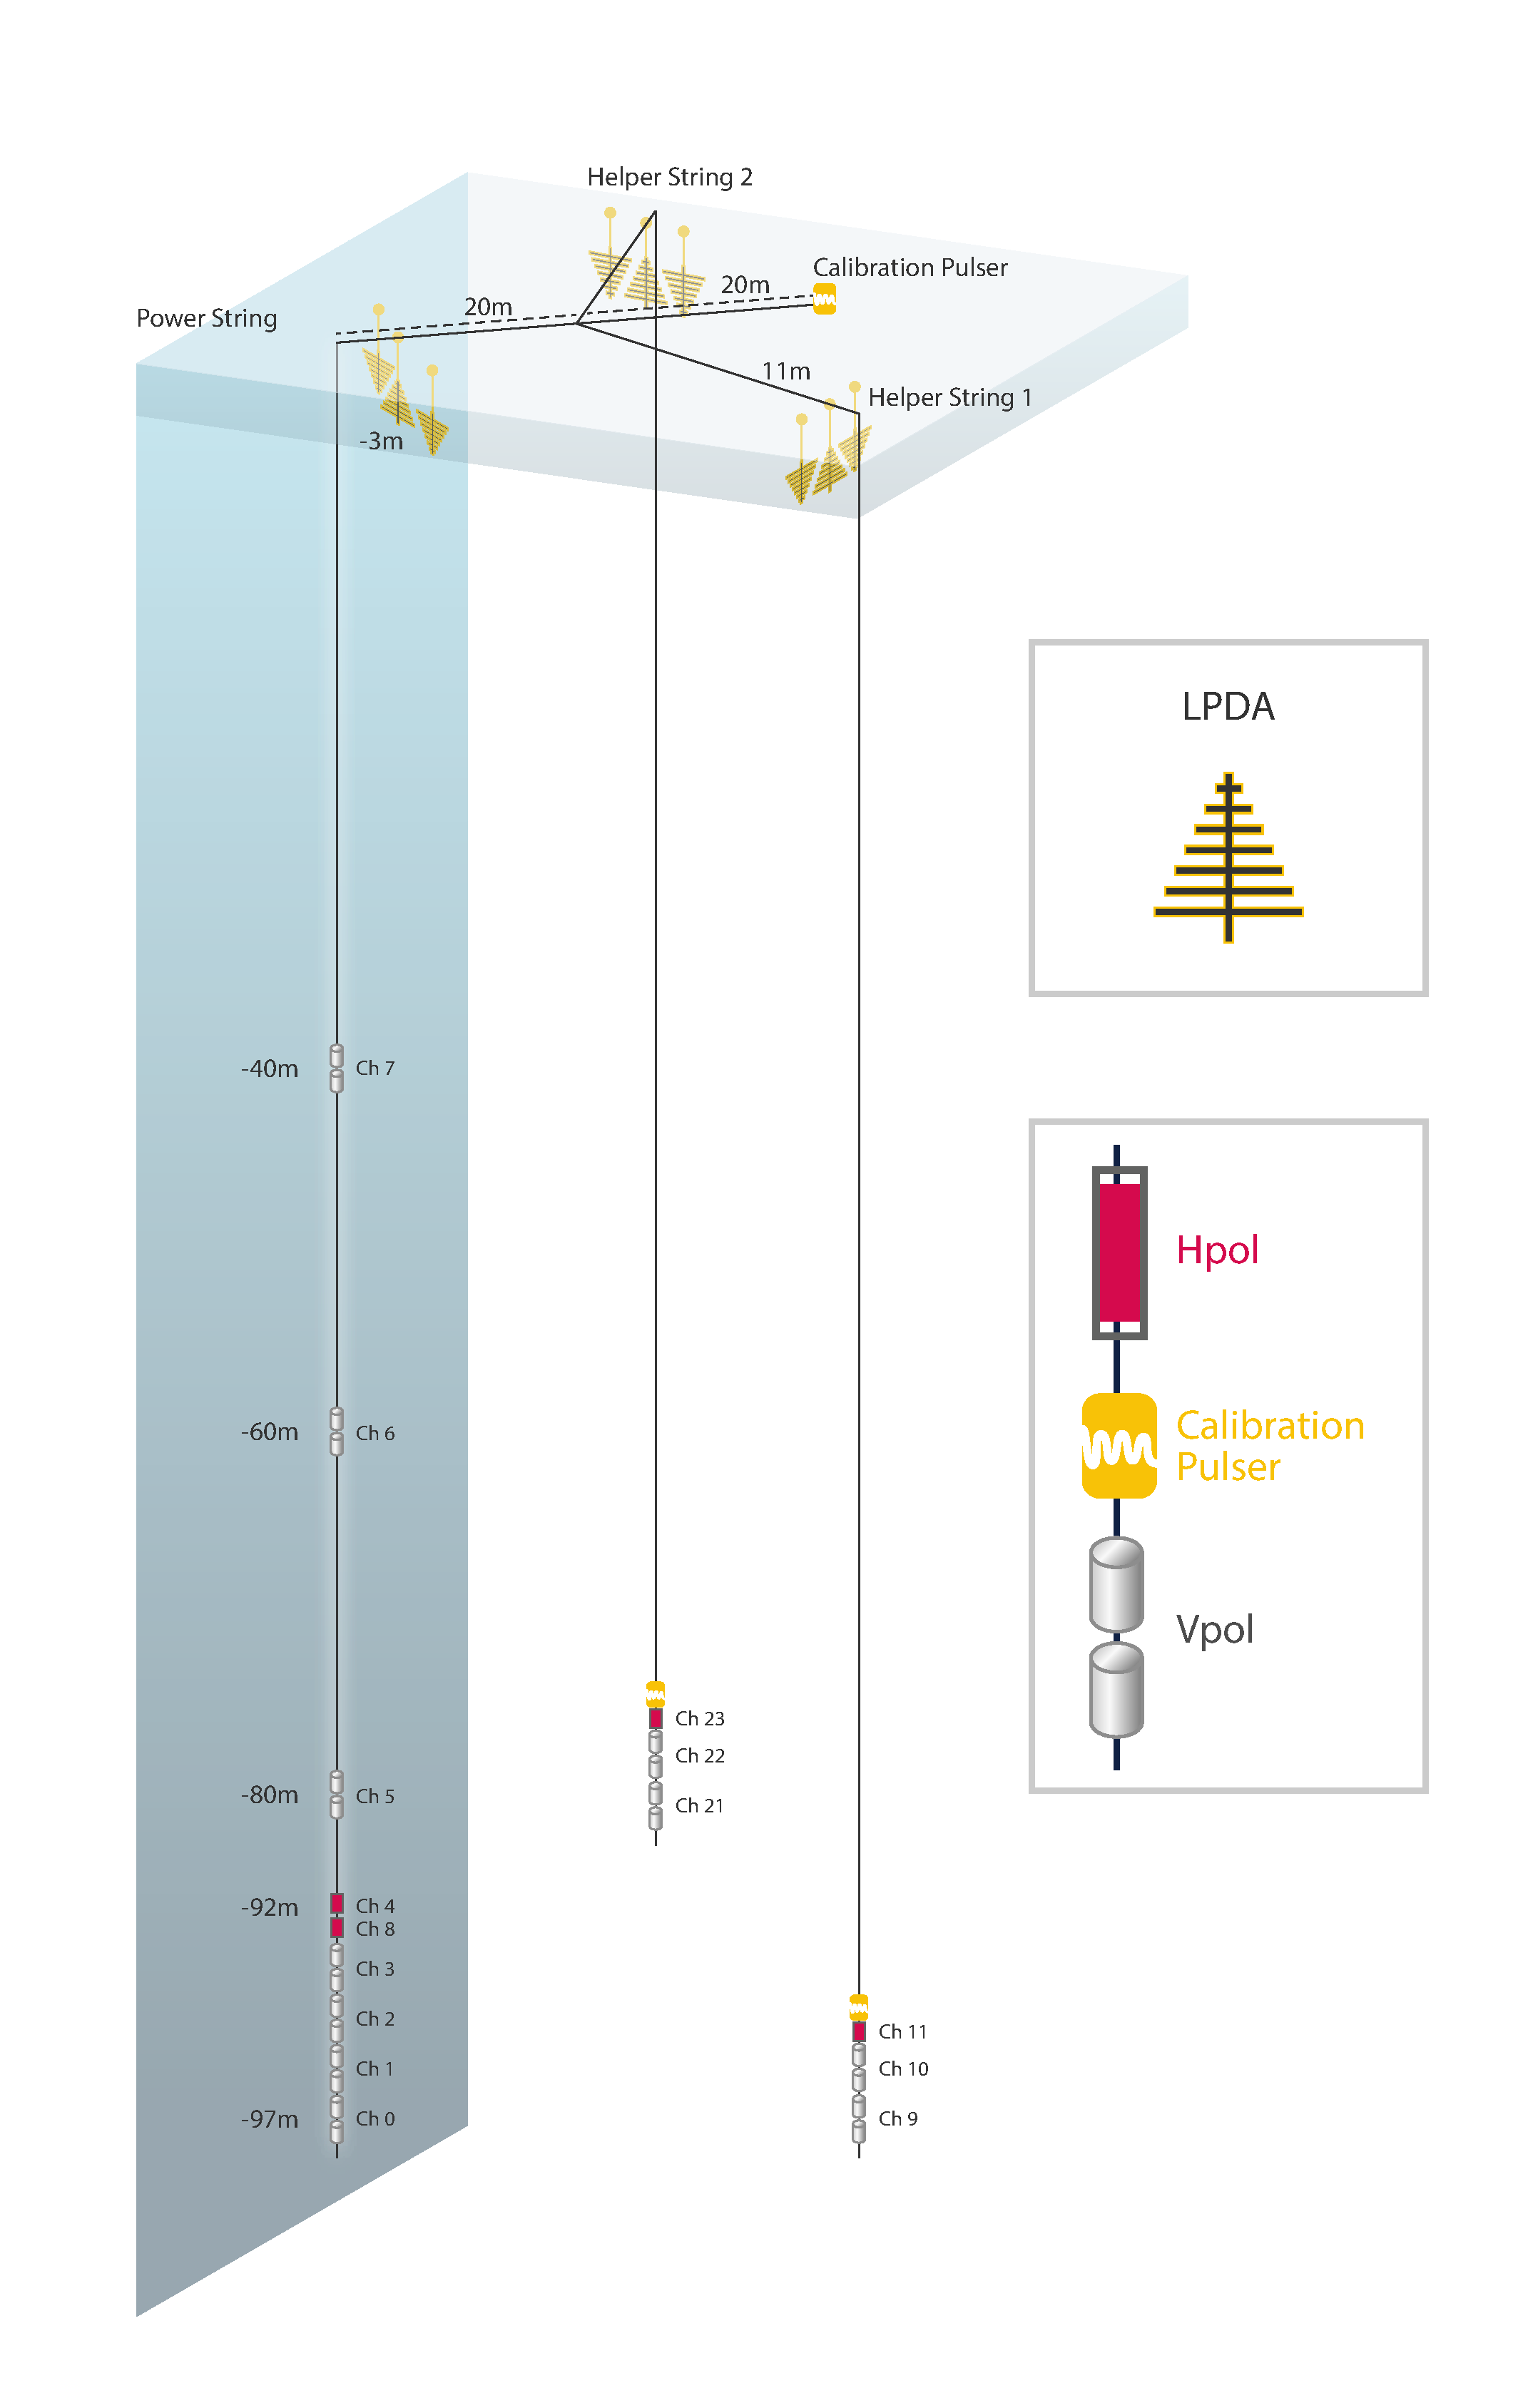
\includegraphics[width=0.9\textwidth]{figures/detector.pdf}	
	\caption{illustration of the detector}
	\label{fig:detector}
\end{figure}
\newpage
The radio signal from a neutrino often travels along both direct and refracted paths (designated DnR) to the deep array, this happens because the upper ice layer is a non-uniform medium where the signal trajectory is bent, as illustrated by a simulation in figure \ref{fig:path_illustration}. 

\begin{figure}[ht]
	\centering
	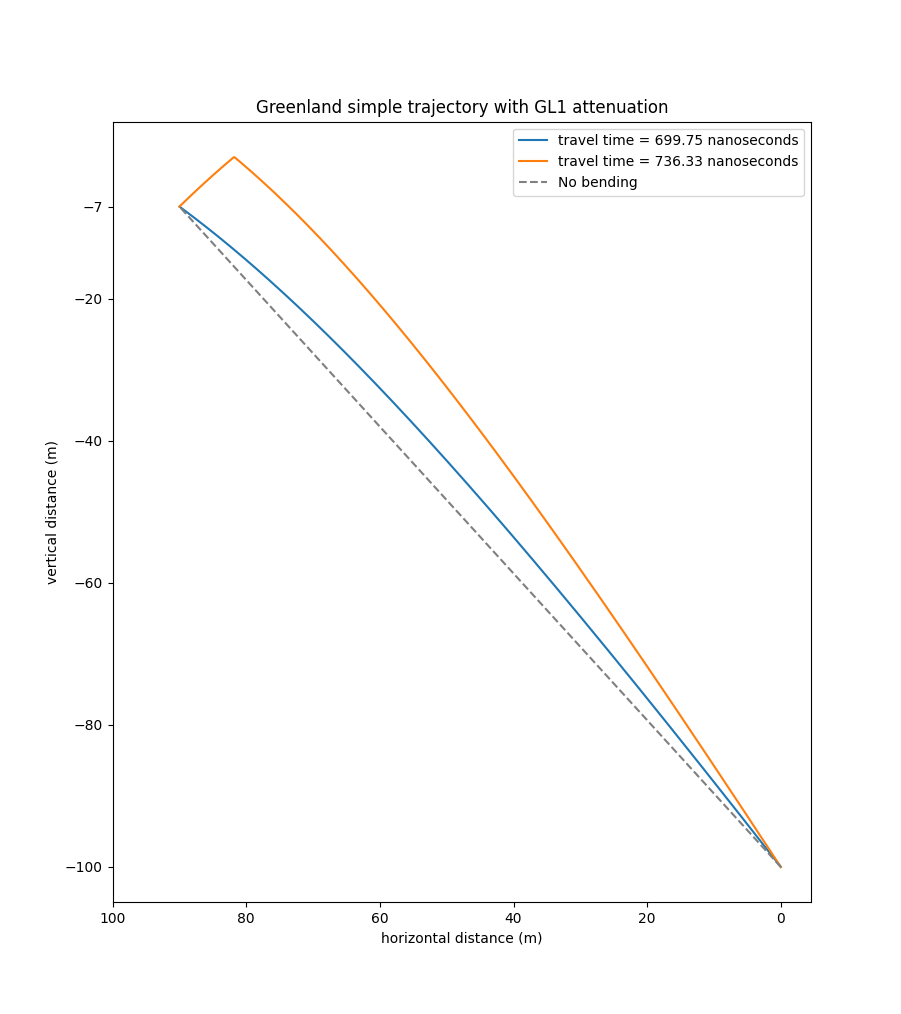
\includegraphics[width=0.6\textwidth]{figures/path_illustration.png}	
	\caption{illustration of a neutrino signal path}
	\label{fig:path_illustration}
\end{figure}


This double pulse characteristic would be a smoking-gun signature of an in-ice source. The two helper strings are needed for a full direction reconstruction. Three independent measurements are needed for azimuthal information, which is provided by the Vpol (Vertical polarization) antennas and placing the Hpol (Horizontal polarization) antennas at different depths on every string, both zentih and azimuth information will be provided for those signals. The helper strings' calibration pulsers, as well as one on the surface, will ensure regular monitoring of the performance of the station and provide information useful for precise calibration of the antenna geometry.

Christoph Welling did an investigation into energy reconstruction from the received signals\cite{Welling_2019} for air showers in one single station (as the RNO-G stations are so far apart this is the case here aswell) and he noticed that it is nescessary to know if the detector who observes an event falls inside or outside the Cherenkov cone to accurately reconstruct the primary particle energy as most over-estimated energies in his simulations are caused by events viewed from within the Cherenkov ring being mistaken for events outside of it. He went on to show that, if we somehow know if the shower was seen from inside or outside the ring from some extra source, that most outliers in the energy disappeared. It is shown by Hiller et al.\cite{Hiller_2017} that the combination of a muon detector with the radio detector might make the issue of confusion between being within or outside of the Cherenkov-ring disappear. Because of this the RNO-G stations are fitted with surface Log Periodic Dipole Antennas (LPDA), capable of detecting muons.
Note that this is for air showers, the radio signal from neutrinos show additional complexities.

\begin{figure}
	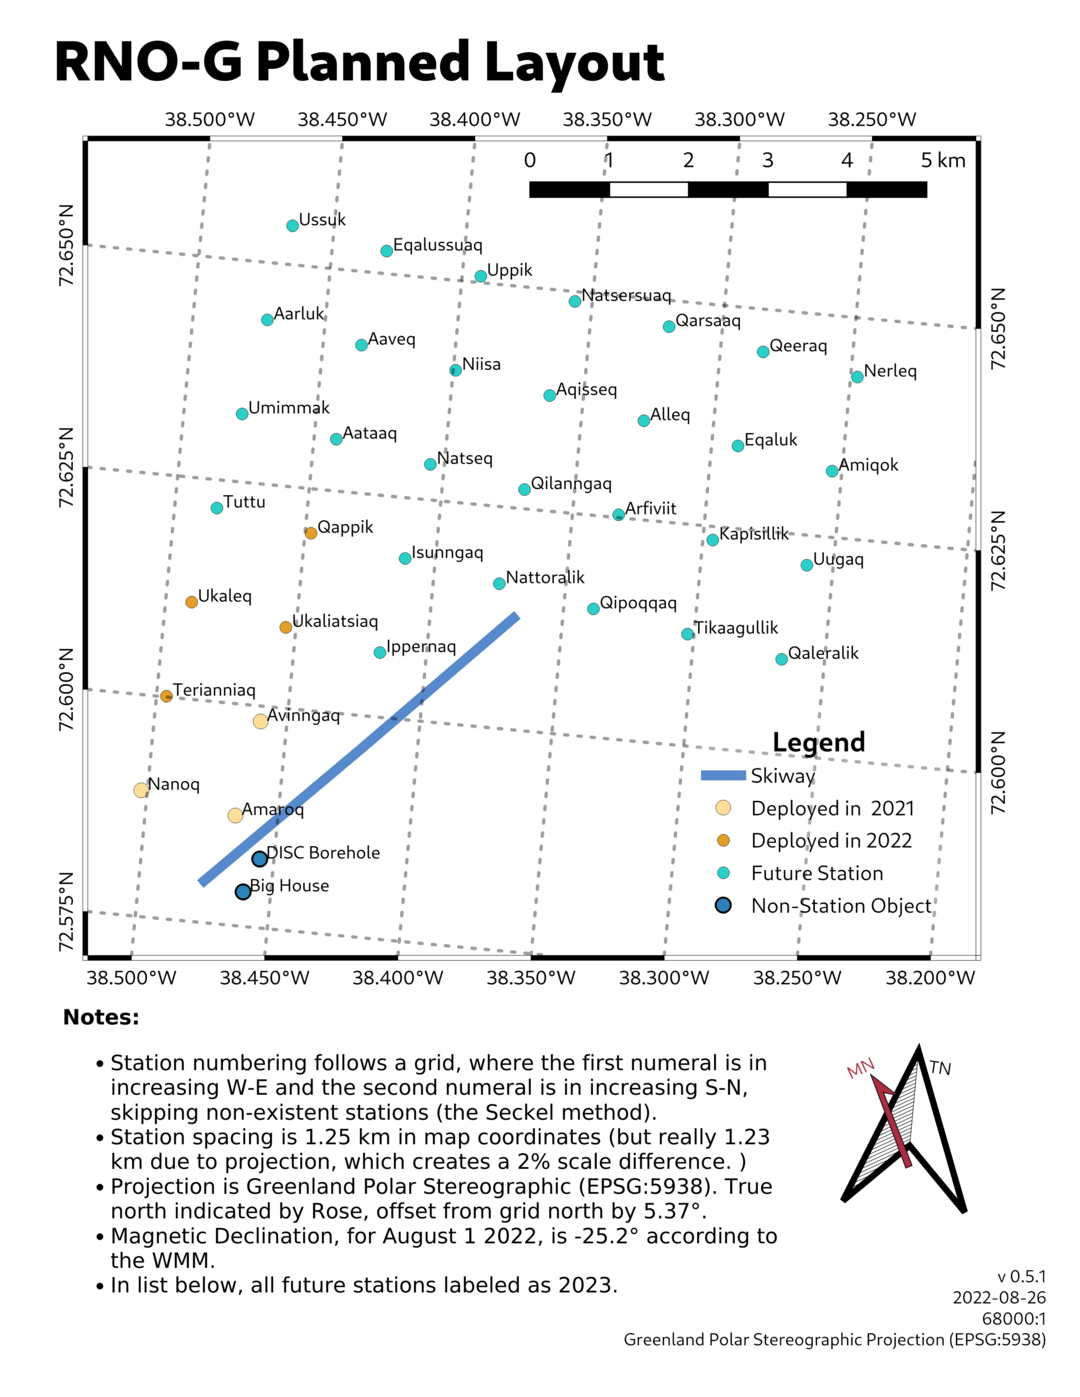
\includegraphics[width=\textwidth]{figures/station-map.png}	
	\caption{map of the station}
	\label{fig:station map}
\end{figure}

% =====================================================================
% End matter
% =====================================================================
\newpage
%----------------------------------------------------------------------------------------
%	REFERENCE LIST
%----------------------------------------------------------------------------------------
\bibliography{sources}
\bibliographystyle{plain}

\end{document}
